\chapter{Design}
This chapter of the report has the purpose of presenting the architecture of the DC-Net simulator from different perspectives through the utilization of UML diagram notations. The overview of the system is still an abstract one, but it is an important step to realize a successful implementation. 

Firstly, the architecture diagrams of the application and examples of the event-based communication will be shown. Following, there is a series of sequence diagrams that exemplifies the data flow between clients and server both for the basic implementation of the protocol and the advanced one.


\section{System Architecture}
The architecture of the simulator is simple.  

\begin{figure}[H]
    \centering
    \fbox{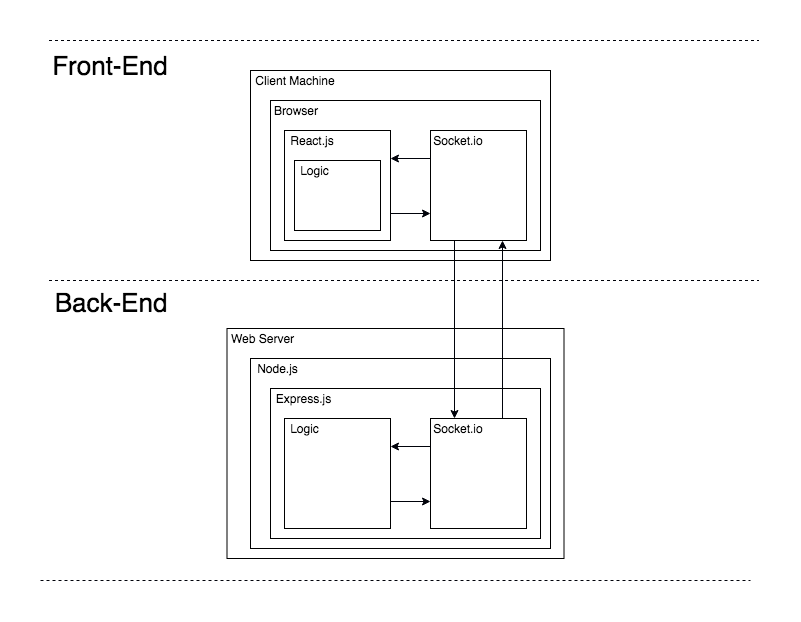
\includegraphics[width=0.9\textwidth]{Images/Design/architecture.png}}
    \caption{System Architecture}
    \label{fig:systemArchitecture}
\end{figure}


\section{Minimal Distributed Architecture}

\begin{figure}[H]
    \centering
    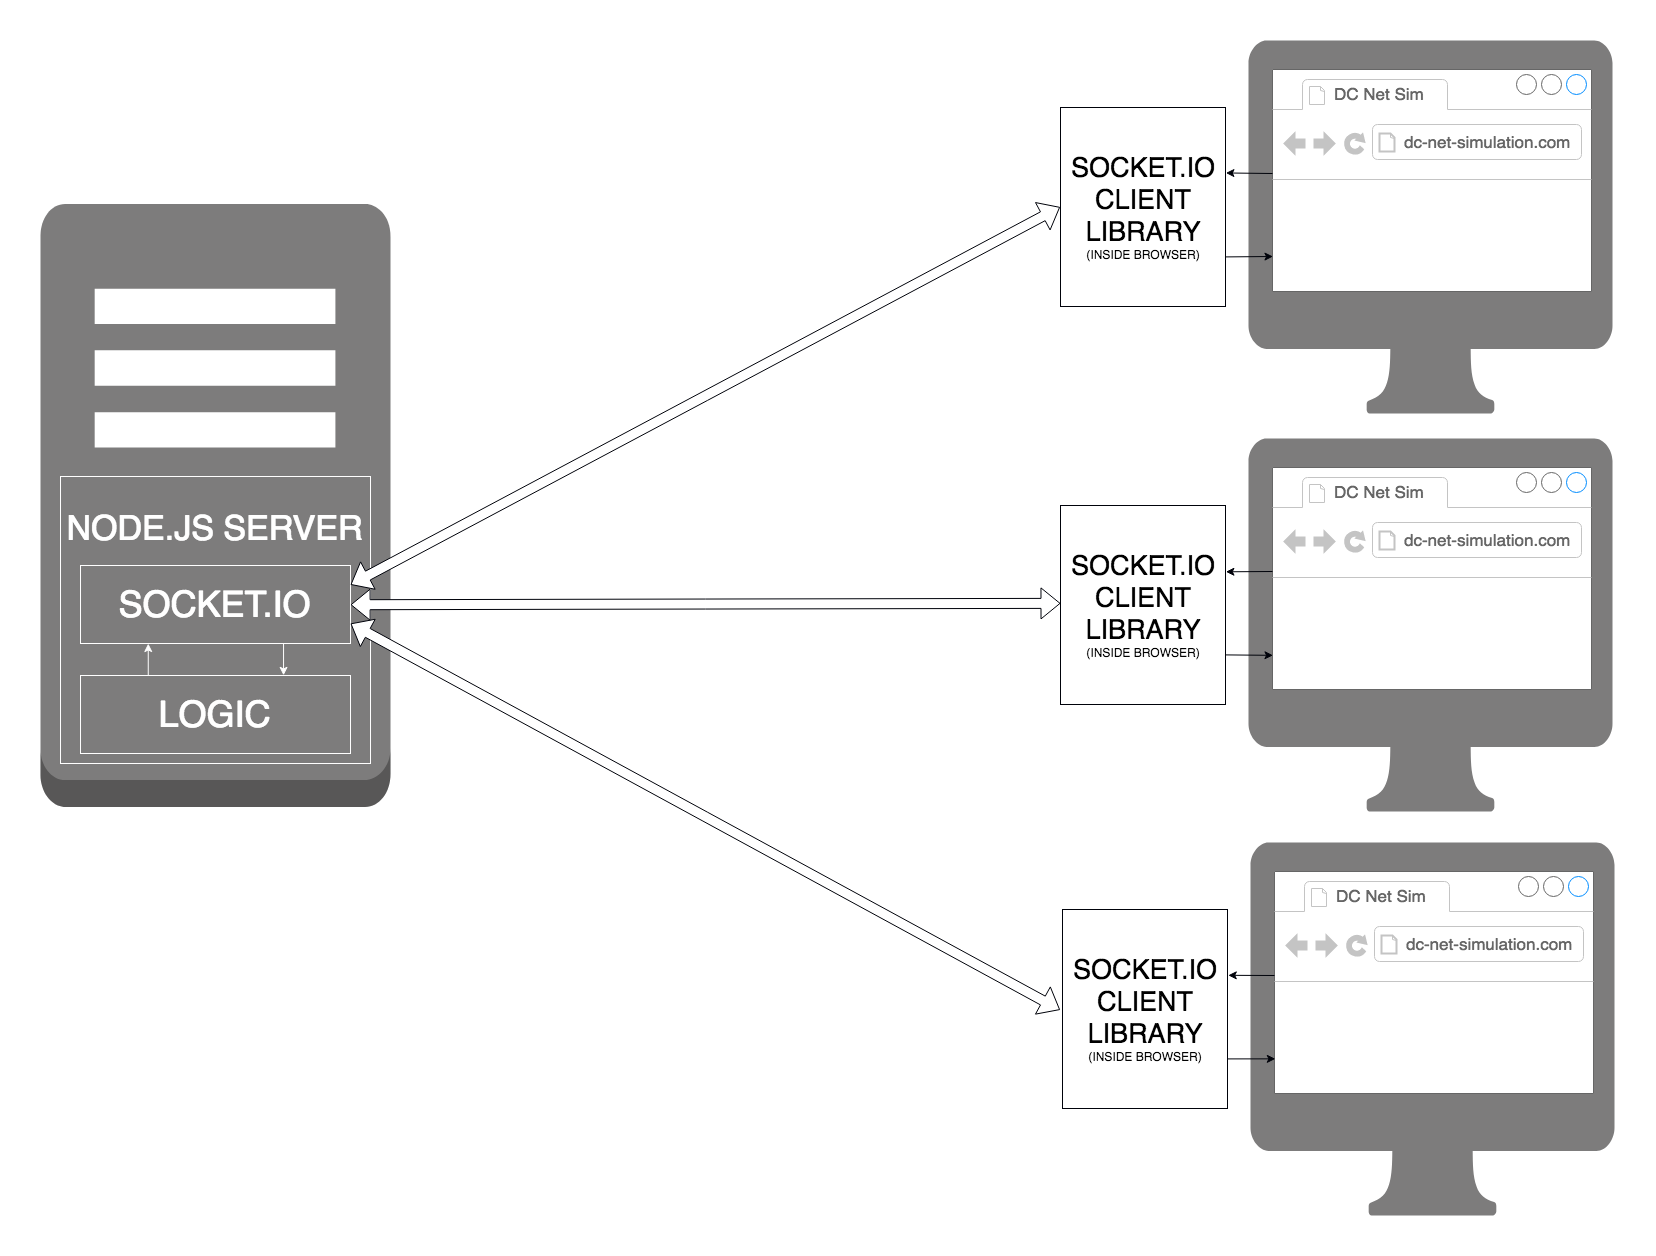
\includegraphics[width=0.8\textwidth]{Images/Design/distributedArchitecture.png}
    \caption{Server with three clients connected}
    \label{fig:distrubtedArchitecture}
\end{figure}


\section{Event-Based Communication Example}
View from single client point of view.

\begin{figure}[H]
    \centering
    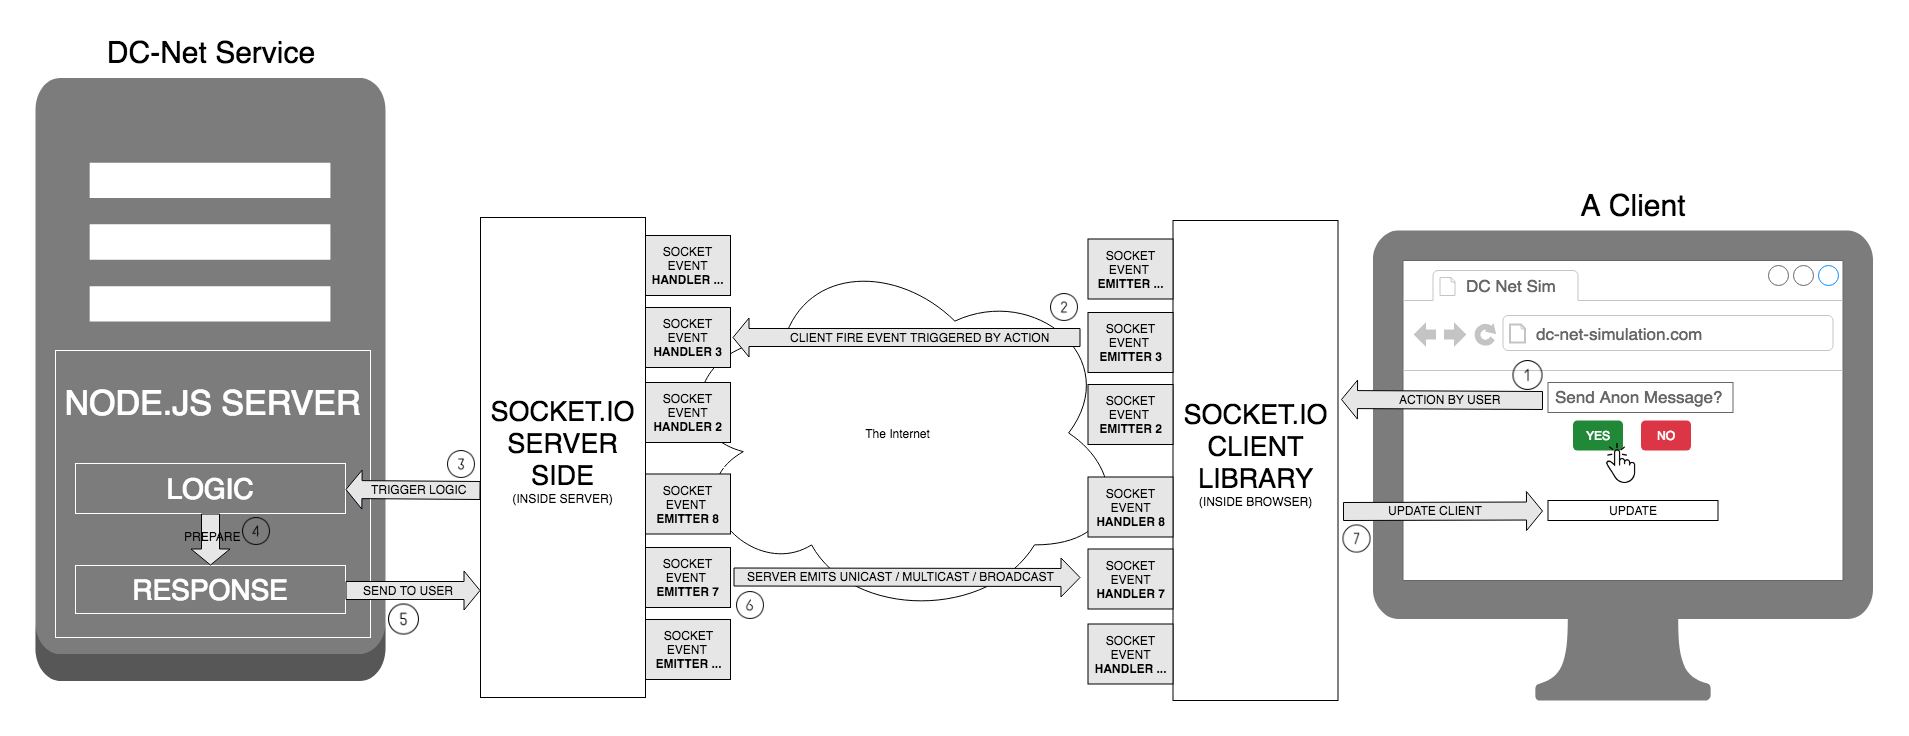
\includegraphics[width=1\textwidth]{Images/Design/singleClientSocketEvent.png}
    \caption{Socket event emission from client example}
    \label{fig:socketEventEmission}
\end{figure}



\section{Data flow depiction through sequence diagrams}


\begin{figure}[H]
    \centering
    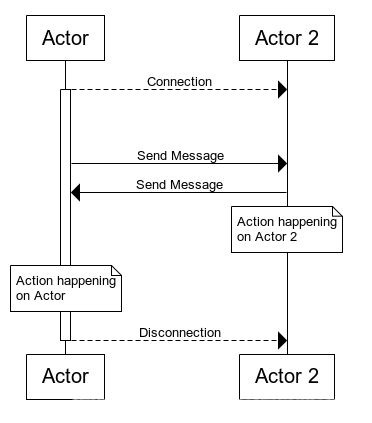
\includegraphics[width=0.5\textwidth]{Images/Design/seqDiagramLegend.png}
    \caption{Sequence Diagram Legend}
    \label{fig:sequenceDiagramLegend}
\end{figure}


\subsection{Basic Data Flow Design}

\begin{figure}[H]
    \centering
    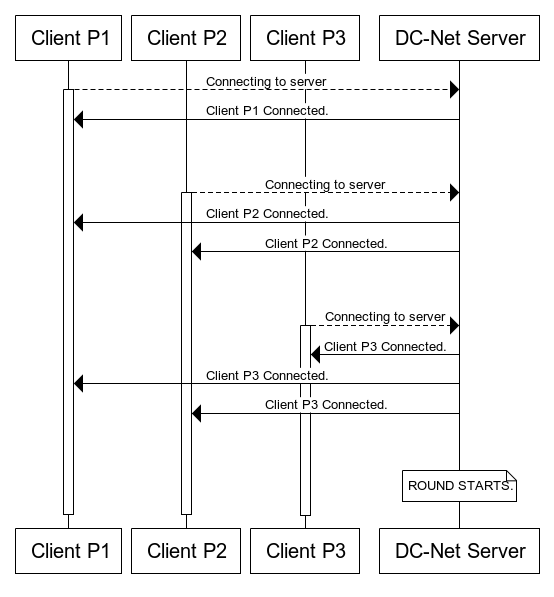
\includegraphics[width=0.7\textwidth]{Images/Design/clientsConnection.png}
    \caption{Connection of three clients needed to start protocol}
    \label{fig:clientsConnection}
\end{figure}

\begin{figure}[H]
    \centering
    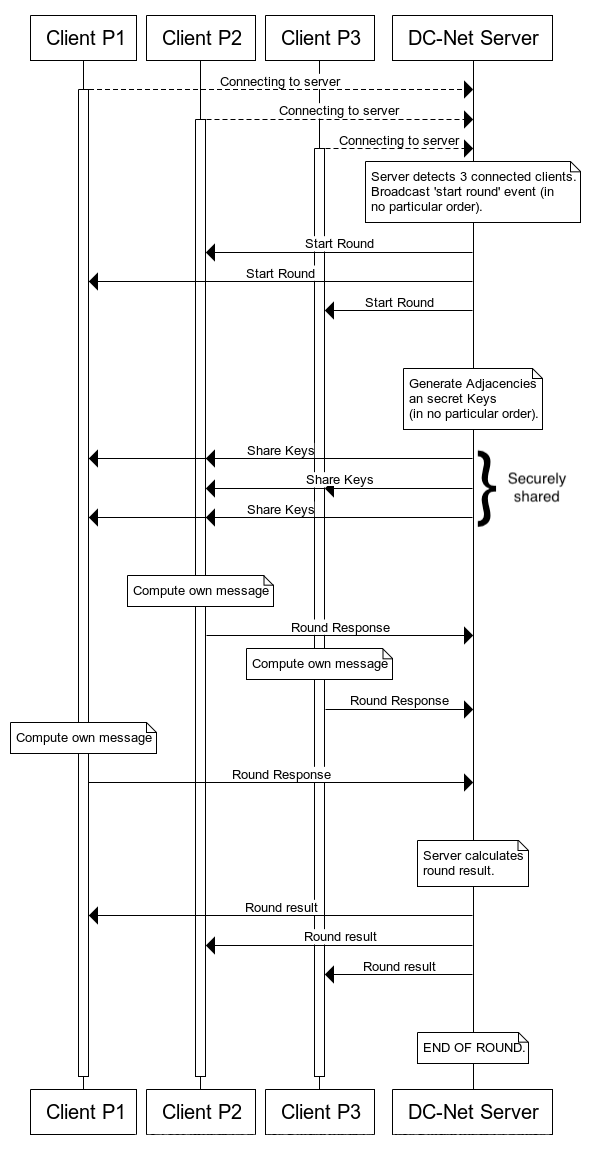
\includegraphics[width=0.8\textwidth]{Images/Design/successfulRound.png}
    \caption{Detailed example of a successful round}
    \label{fig:successfulRound}
\end{figure}

\begin{figure}[H]
    \centering
    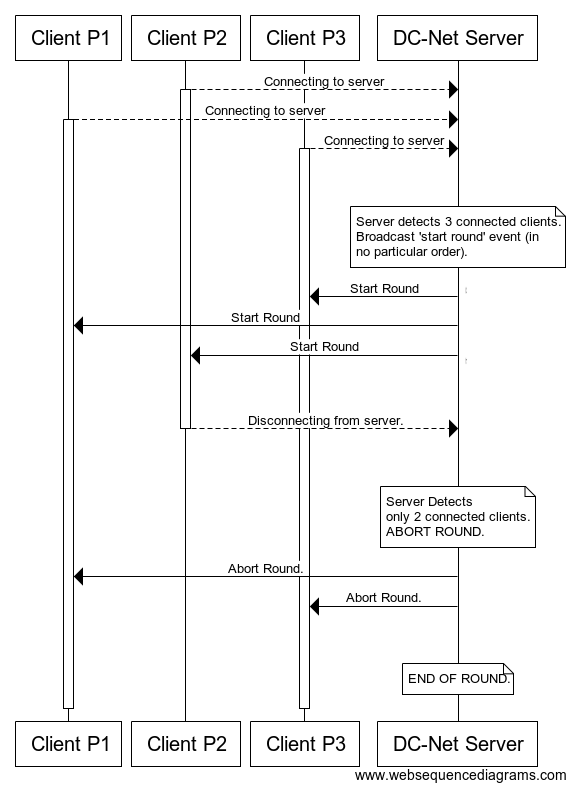
\includegraphics[width=0.7\textwidth]{Images/Design/abortedRound.png}
    \caption{Detailed example of aborted round}
    \label{fig:abortedRound}
\end{figure}

\begin{figure}[H]
    \centering
    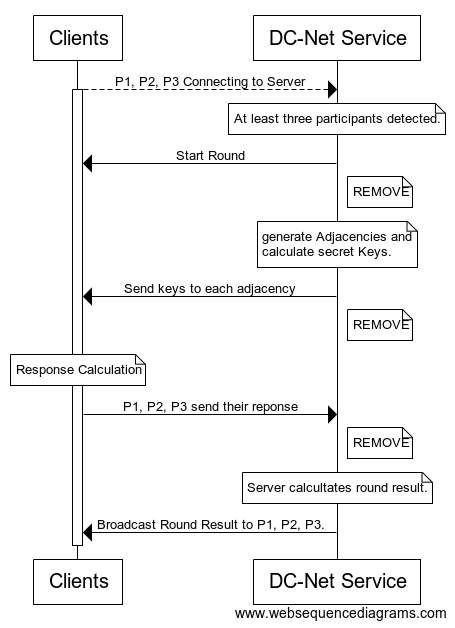
\includegraphics[width=0.7\textwidth]{Images/Design/singleRoundCondensed.png}
    \caption{Concise representation of a single round }
    \label{fig:singleRoundCondensed}
\end{figure}


\subsection{Advanced Data Flow Design}


\begin{figure}[H]
    \centering
    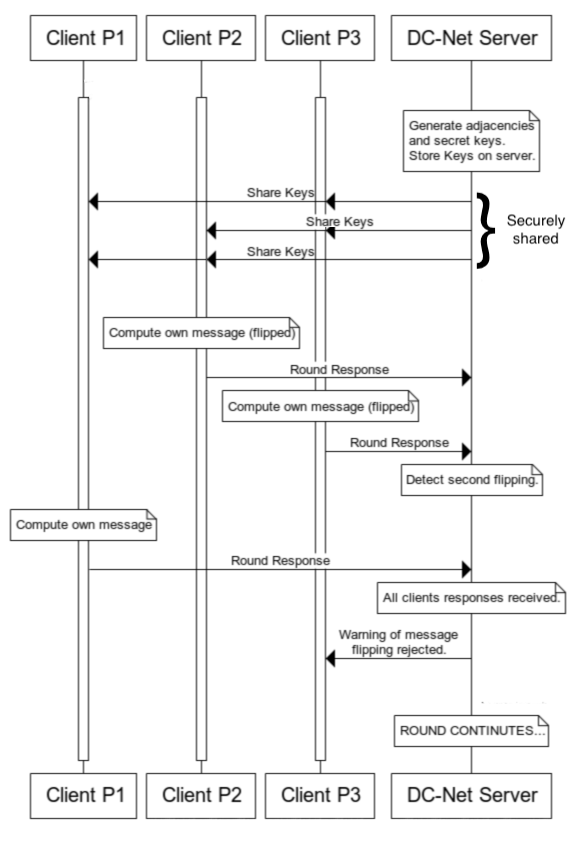
\includegraphics[width=0.6\textwidth]{Images/Design/collisionDetection.png}
    \caption{Detecting message collision}
    \label{fig:collisionDetection}
\end{figure}

\begin{figure}[H]
    \centering
    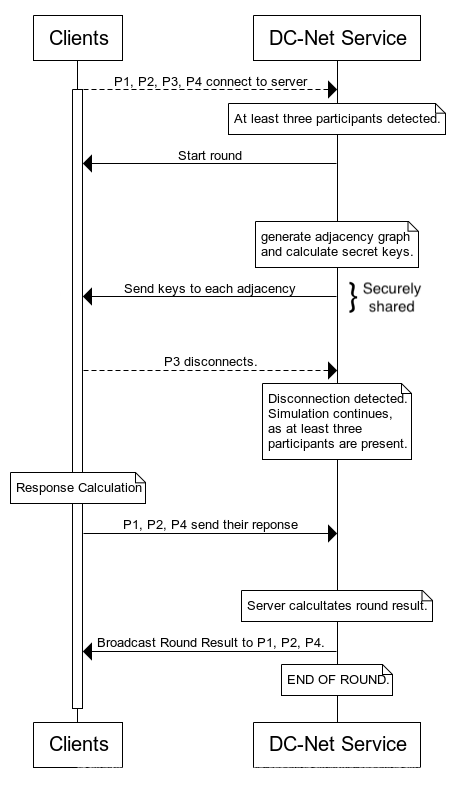
\includegraphics[width=0.5\textwidth]{Images/Design/roundWithDisconnections.png}
    \caption{Round performed with disconnecting client}
    \label{fig:roundWithDisconnections}
\end{figure}

\begin{figure}[H]
    \centering
    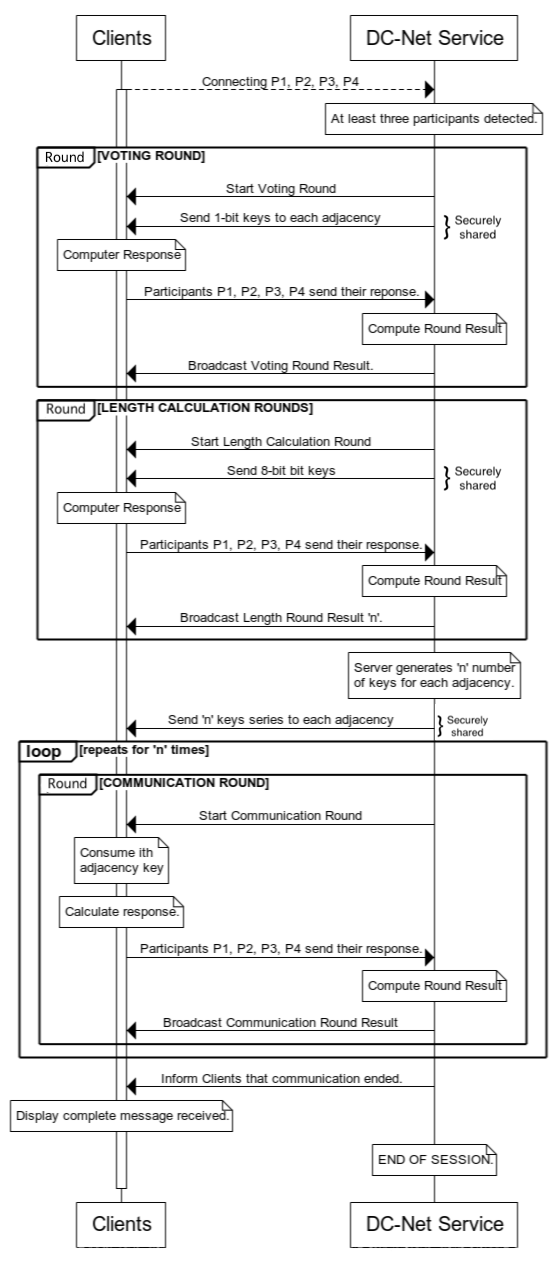
\includegraphics[width=0.6\textwidth]{Images/Design/longRound.png}
    \caption{Representation of complex round of communication}
    \label{fig:longRound}
\end{figure}